\tikzset{every picture/.style={scale=.55}}
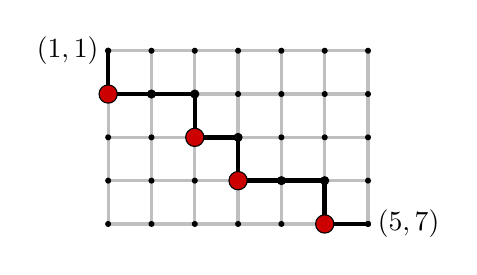
\begin{tikzpicture}
\draw[gray!50, very thick] (0,0) grid (6,4);
\foreach \i in {0,...,6}
    \foreach \j in {0,...,4}
        \fill (\i,\j) circle (2pt);
\draw[ultra thick] (0,4) -- (0,3)--(2,3)--(2,2)--(3,2)--(3,1)--(5,1)--(5,0)--(6,0) ;
\fill[black]  
(1,3) circle (3pt)
(2,3) circle (3pt)
(2,2) circle (3pt) 
(3,2) circle (3pt) 
(3,1) circle (3pt) 
(4,1) circle (3pt) 
(5,1) circle (3pt) 
(5,0) circle (3pt);

\path [draw=black, fill=red!80!black]
(0,3) circle (6pt) 
(2,2) circle (6pt)
(3,1) circle (6pt)
(5,0) circle (6pt);           
\fill[black] 
(0,4) circle (2pt) node[left] {$(1,1)$} 
(6,0) circle (2pt) node[right] {$(5,7)$};
\end{tikzpicture}